\documentclass[12pt]{article}
\usepackage[utf8]{inputenc}
\usepackage{graphicx, latexsym, amsmath, amssymb, amsthm}
\usepackage{multicol}
\usepackage{geometry}
 \geometry{
 a4paper,
 total={170mm,257mm},
 left=16mm,
 top=10mm,
 }

\graphicspath{{../apps/aco_tsp/test/results/}}
\title{Ant Colony Optimization in Elixir}
\author{Andrea Malleo}
\begin{document}

\maketitle
\section{Abstract}
In this paper we present a distributed implementation of an Ant Colony Optimizer 
for the Travelling Salesman problem using the Actor Model of Concurrency. We give
an overview of the system architecture and present the experiments we ran to validate 
the correctness of the code and compare performance against an open source serialized 
implementation. We find that performance compared to the serialized approach scales 
with the problem size, and identify key future enhancements for further speed up.

%\begin{multicols*}{2}

\section{Introduction}Ant Colony Optimization \cite{Dorigo1997AntCS} is a bio-inspired coorperative learning algorithm for 
    finding the shortest path in a graph. Ants are simulated as software agents who 
    independently travel along the graph, dropping pheromones in their wake that 
    evaporate with time. These pheromones are a form of communication for other ants in
    the colony, as concentration of pheromones on a pathway signals recent concentration of other ants
    in this same spot.

    After each round, the individual solutions for the ants are agregated and the optimal choice
    from all of the candidates is selected. 
    Additionally the shared pheromone matrix, acting as a collective and evolving intelligence 
    for the colony of ants, is updated to reflect new pheromone concentrations following all of the 
    ant tours of this round.  In successive rounds of the algorithm, ants bias their path 
    toward edges with higher pheromone concentration. Since edges of greater distance take 
    longer to travel, evaporation will lower the concentration of pheromone there and make 
    future ants less likely to take those edges. Over successive rounds, the searches converge
    to some (locally) optimal solution. 
    There have since been many enhancements to the original Any Colony algorithm,
    such as the Ant Colony System \cite{Dorigo1999AntCO} and the Max-Min Ant System \cite{maxMin} 
    which producer better convergence results. In this paper we stuck with original simplest 
    approach and settled for convergence to some local minimum which empirically proved to be 
    not too far from the global minimum.\\

    The problem being considered here is the Travelling Salesman Problem \cite{wikiTSP},
    that is to find a complete tour of a fully connected graph with the minimal 
    cost.


\section{Related work}
The independence of the ant agents lends the algorithm to parallelization. 
The central point of synchronization is the pheromone matrix, which must 
maintain accurate values for a given round and update atomically for the 
next round. Many approaches have been presented that parallelize the algorithm 
in different ways. Pedemonte et. al \cite{SurveyParallel} categorize 
the approaches, drawing distrinctions between a *master-slave model*
with the simultaneous execution of ants providing updates to 
a master process maintainting the global pheromone matrix and a
*parallel independent runs model* where many
executions of independent ACO systems run simultaneously,
further subdivided between
whether or not the independent colony systems eventually coordinate
 with each other. 
There are also GPU based implementations, such as in \cite{GPU}.
\\

Instead of working under the shared memory model of distributed 
computing, Ilie and Badica
reformulate the classical algorithm using message 
passing in a multi-agent framework  in \cite{multiagent}.
Their work leverages existing multiagent system middleware, but the paradigm
shift they introduced is built up on by Starzec et all in \cite{star1}.
Here they build an actor model\cite{ActorModel} implementation
using Akka, a toolkit for building concurrent message driven applications 
for Scala. Their paper outlines a hierarchy of processes in their architecture,
the bottom layer, representing ants, being the most ubiquitous, with each 
layer of managers collecting and aggragating state updates from the layer
beneath it. It is this paper the main work of this paper is based.
The process architecture is largely the same, although a bit simplified 
as will be discussed towards the end of the Methods and in Future work. 
Novel to our approach is the choice of Elixir as the high level programming
language for implementation. Elixir too employs the Actor computation model and 
thus uses message passing as a lock free form of state synchronization.

\section{Methods}
This section will outline the construction of this implementation by considering
in turn the five process types running in the ACO system:
 \begin{itemize}
    \item the ant: responsible for graph traversals according to probablistic rules
    \item the graph manager: responsible for servicing requests for graph state
    \item the pheromone manager: responsible for servicing requests for pheromone matrix state
    \item the ant manager: responsible for collecting ant solutions and reporting the optimal one
    \item the colony manager: maintains global optimal solution
 \end{itemize}
The most ubiquitous of these at runtime is the ant process. At the start 
of each round, an ant begins at a randomly selected node. The following 
logic loops until a complete tour of the graph is completed.
At the topic of the loop the Ant is at some given node.  
The Ant requests from  the Graph Manager process the set of possible 
edges emanating from this node (given the list of nodes already traversed 
in this tour) and waits for the response. If the 
response indicates that the tour of the ant is complete, the ant 
sends up its Solution Report (the order its nodes and the cost) to both the
 Pheromone Manager 
and the Ant Manager and then transitions into the next round. Otherwise,
the Edge Response will include the list of edges left and their respective costs.
The ant then forms a Pheromone Request for this set of edges and sends it to the Pheromone Manager.
Following a response, the Ant will compute the probability distribution over the set of edges
emanating from node i to node j as: 
\begin{flalign*}
    p_j(t) = \frac{[\tau_{ij}(t)]^{\alpha} [\eta_{ij}(t)]^{\beta} }{\Sigma_{k \in \text{edges}} [\tau_{ik}(t)]^{\alpha} [\eta_{ik}(t)]^\beta}
\end{flalign*}
where $\tau_{ij}(t)$ is the intensity of the pheromone trail on edge $ij$ 
and $\eta_{ij}$ is the reciprocal of the cost of edge $ij$. The ant then draws an edge from this distribution
and makes its move, before the cycle repeats once more. 

The Graph Manager holds the graph: a dictionary with node numbers as keys, mapping to 
a dictionary holding key, value pairs of every other node and the cost of this edge 
between the two. Note that the graphs on which the Travelling Salesman Problem is run 
are complete, so space requirement is $n^2$ in the number of nodes. 
The Graph Manager loop simply services Edge Requests that come in, first checking
to see for a completed tour, and otherwise pulling up the total set of neighbors 
and edge costs for a given node and dropping from this set any nodes already visited
in this tour. Note that the state contained in the Graph Manager is constant 
and therefore valid indefinitely. As such, it needn't care about which ant 
is making a request or what state that ant is in.  

This differs significantly from the Pheromone Manager. Recall that the 
end of every complete tour, the ant sends up the order of its nodes 
and the tour cost to the Pheromone Manager. This is so that the ant's
pheromones may be sprinkled along its trail. Precisely, for ant k,
the pheromone contributions to an edge $ij$ for a given round is 
\begin{flalign*}
    \Delta \tau_{ij} = \begin{cases}
        \frac{Q}{C_k} & \text{if kth ant uses edge (i,j)} \\
        0 & \text{otherwise}\\
    \end{cases}
\end{flalign*}
Where Q is a parameter, set to 1 here, and $C_k$ is the cost of 
the tour for ant k.
The Pheromone Manager must only service requests for the pheromone matrix for 
a given round $m$ and simultaneously collect the completed tour reports from all 
of the ants in order to compute the pheromone matrix for round $m+1$. To 
enforce this, Requests and Reports contains a field for the round number,
and the Pheromone Manager will drop any Pheromone Requests or Solution Reports 
from the ants marked for a different round from the Manager's.
The Pheromone Manager counts how many Solution Reports it has 
received in any round, and once one from each ant has come in, the pheromone matrix 
needs to be updated atomically for the next round.\\

As a time saving optimization, there 
are actually two pheromone matrices kept by the Manager, the first is the live one for 
the current round, and the second is the working matrix for the next. As tours
come in, the pheromone contributions are accumulated for all of the edges in the 
working matrix, while the live matrix remains valid for interleaved Pheromone Requests
coming in. Once it is time to transition to the next round, the live 
pheromone matrix is updated for each edge $ij$ as 
\begin{flalign*}
    \tau_{ij}(t+1) = \rho \tau_{ij}(t) + \Sigma_{k=1}^n \Delta \tau^k_{ij}
\end{flalign*}
where $\rho$ represents the pheromone decay parameter and the 
sum is over all $n$ ants. Note that if a Request or Solution comes in from an ant 
for the wrong round, it is simply dropped on the floor, and the ant will wait 
five seconds before resending the message. The Pheromone Manager's round increment 
serves as barrier that keeps the independent ant processes from progressing 
with too much variance.

The second process collecting Solution Reports from ants is the Ant Manager. 
In a similar fashion as just described, the Ant Manager only accepts Solutions 
indexed by the correct round, tracking the lowest cost tour received by any 
of the ants, and reporting the final best result up the hierarchy to the Colony Manager.

Finally there is the Colony Manager. In the current state the Colony Manager simply 
reports and saves each new lowest cost solution as it comes in from the Ant Manager.
Future Work will address how its responsibilities might be increased.
\section{Experiments}
Instances of the problem for testing were taken from TSPLIB95 \cite{tsplib95}, 
    an open source repository for TSP benchmark problems.

\begin{figure}
    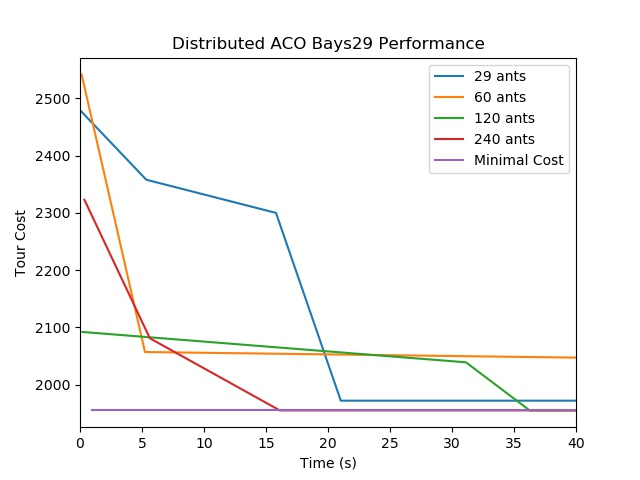
\includegraphics[scale=0.5]{bays29_performance_vs_ants.jpg}
    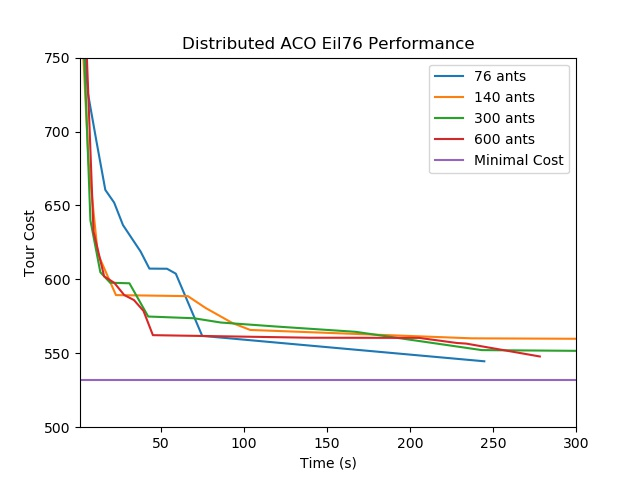
\includegraphics[scale=0.5]{eil76_performance_vs_ants.jpg}
    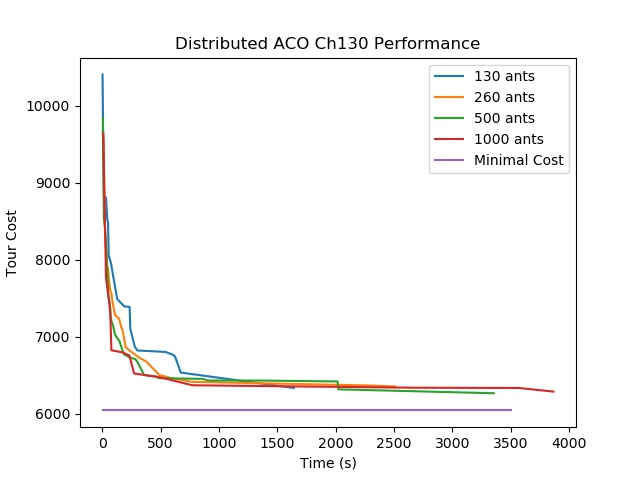
\includegraphics[scale=0.5]{ch130_performance_vs_ants.jpg}
    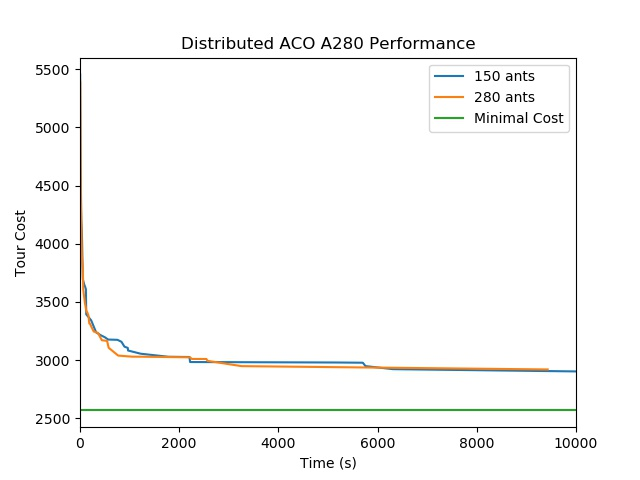
\includegraphics[scale=0.5]{a280_performance_vs_ants.jpg}
\end{figure}


\begin{figure}
    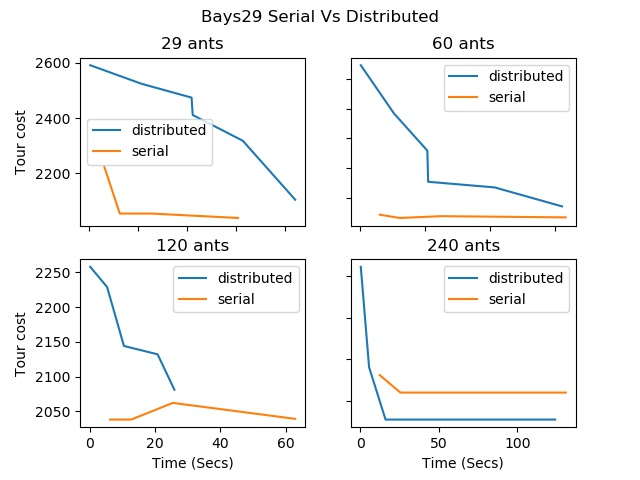
\includegraphics[scale=0.5]{bays29_serial_vs_dist.jpg}
    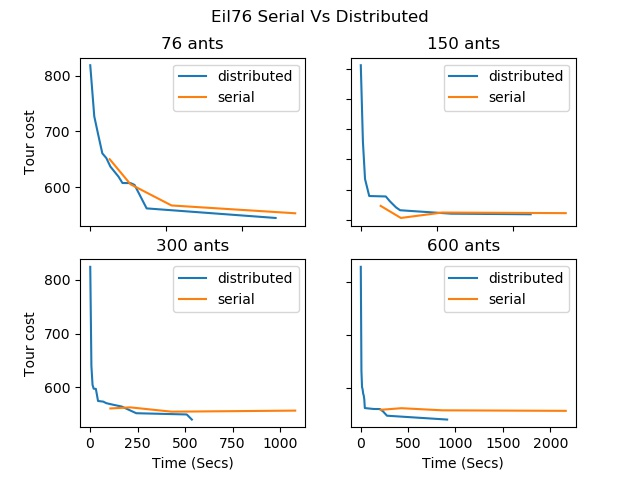
\includegraphics[scale=0.5]{eil76_serial_vs_dist.jpg}
    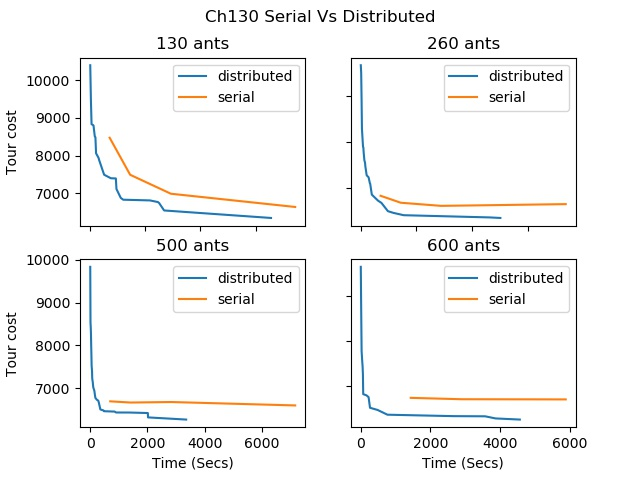
\includegraphics[scale=0.5]{ch130_serial_vs_dist.jpg}
    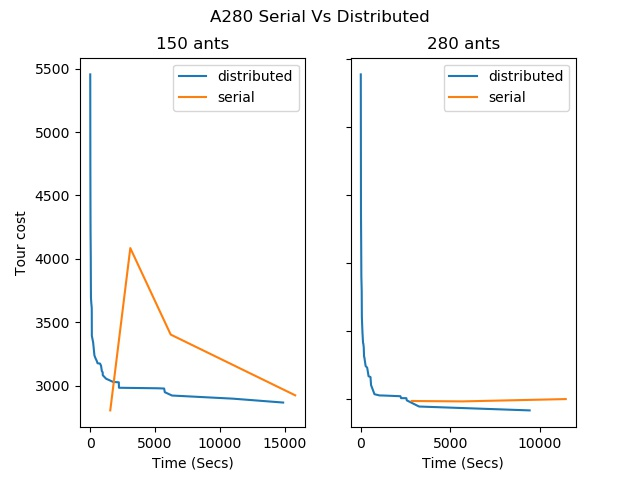
\includegraphics[scale=0.5]{a280_serial_vs_dist.jpg}
\end{figure}

\section{Future Work}
\section{Conclusion}

%\end{multicols*}

\bibliographystyle{plain}
\bibliography{refs}


\end{document}
